\documentclass{article}
\usepackage{amsmath}
\usepackage[a4paper, total={7in, 10in}]{geometry}
\usepackage{graphicx} % Required for inserting images
\usepackage{fontspec}
\setmainfont{David CLM}
\usepackage{amssymb}
\usepackage{chngcntr} % For controlling equation numbering within align*
\counterwithin{equation}{section}
\usepackage{cellspace}
\setlength\cellspacetoplimit{0.3em}
\setlength\cellspacebottomlimit{0.3em}
\addparagraphcolumntypes{S}
\usepackage{multicol}
\usepackage{enumitem}

% these packages must be loaded last 
\usepackage{polyglossia}
\setdefaultlanguage{hebrew}
\setotherlanguage{english}
\usepackage{bidi}

\usepackage{unicode-math}

\title{קוונטים 2 - תרגיל נומרי}
\author{דוד שם־טוב}

\begin{document}

\maketitle

\section{הכנת הקוד}
\stepcounter{subsection}
\subsection{חישוב נומרי עבור מצב היסוד של ${}^{1}\!H$ ($l=0$)}
הנתונים של המערכת הם:
\begin{multicols}{3}
    $\mu = 322.678 MeV / c^2$ \\
    $R_y = 8.592e-03 MeV$ \\
    $a_B = 83.802 fm$ \\
    $V(r) = -\frac{\alpha Z \hbar c}{r}$ \\
    $N = 10000$ \\
    $R = 10\cdot a_B = 838.015 fm$
\end{multicols}
עבור חישוב בשיטת נומרוב:
$$u_{k+1} = \frac{\left[2-\frac{5}{6}\Delta^2W_k\right]u_k-\left[1+\frac{1}{12}\Delta^2W_{k-1}\right]u_{k-1}}{1+\frac{1}{12}\Delta^2W_{k+1}}$$
כאשר 
$$W_k = \frac{2\mu}{\hbar^2}\left(E-V\left(r_n\right)\right) - \frac{l(l+1)}{r^2}$$
עבור האנרגיות $ E = -0.9 R_y, -0.95 R_y, -1.0 R_y, -1.05 R_y, -1.1 R_y$ מתקבלות התוצאות הבאות:

\begin{figure}[h]\label{fig:1.2}
    \centering
    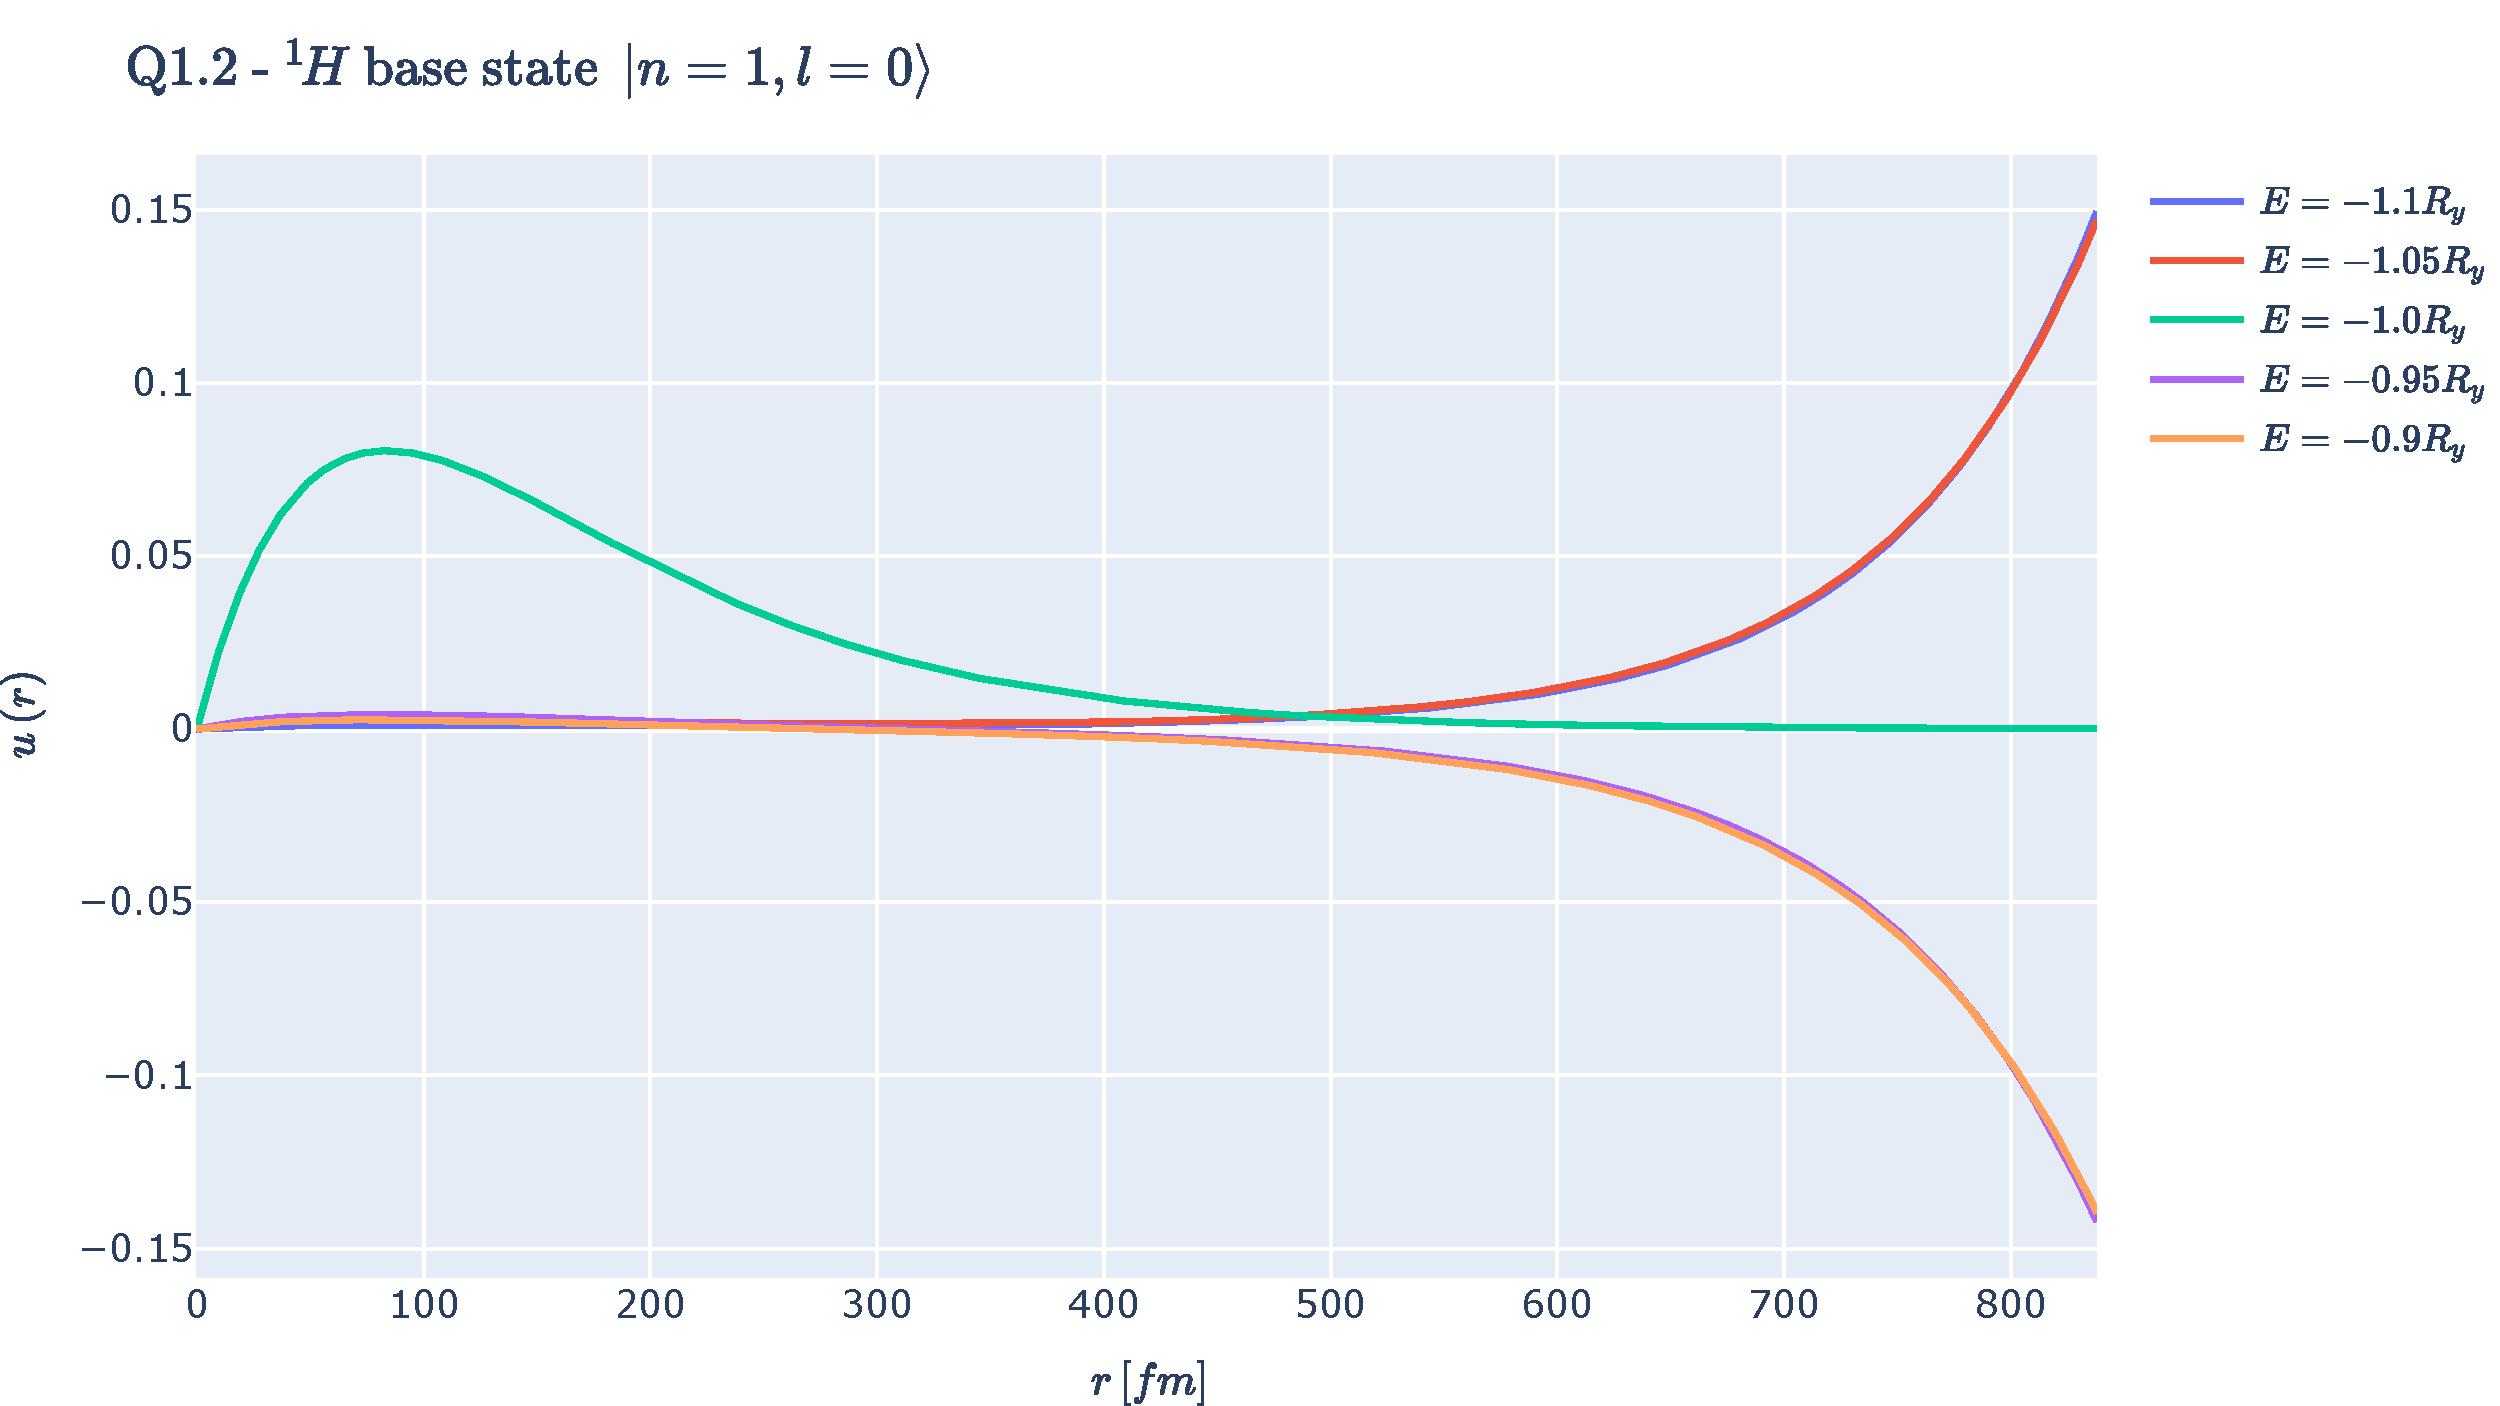
\includegraphics[width=\linewidth]{plots/1.2.pdf}
    \caption{התוצאות עבור אנרגיות שונות}
\end{figure}
ניתן לראות שרק עבור $E = -1 R_y$ הפתרוןדועך ל־0 באינסוף.

\subsection{מציאת שורשים}\label{subsec:1.2}
עבור חיפוש בתחום $-1.05 < \frac{E}{R_y} < -0.95$ נמצא שורש ב־$E = -0.999998 R_y$.
\begin{figure}[h]\label{fig:1.3}
    \centering
    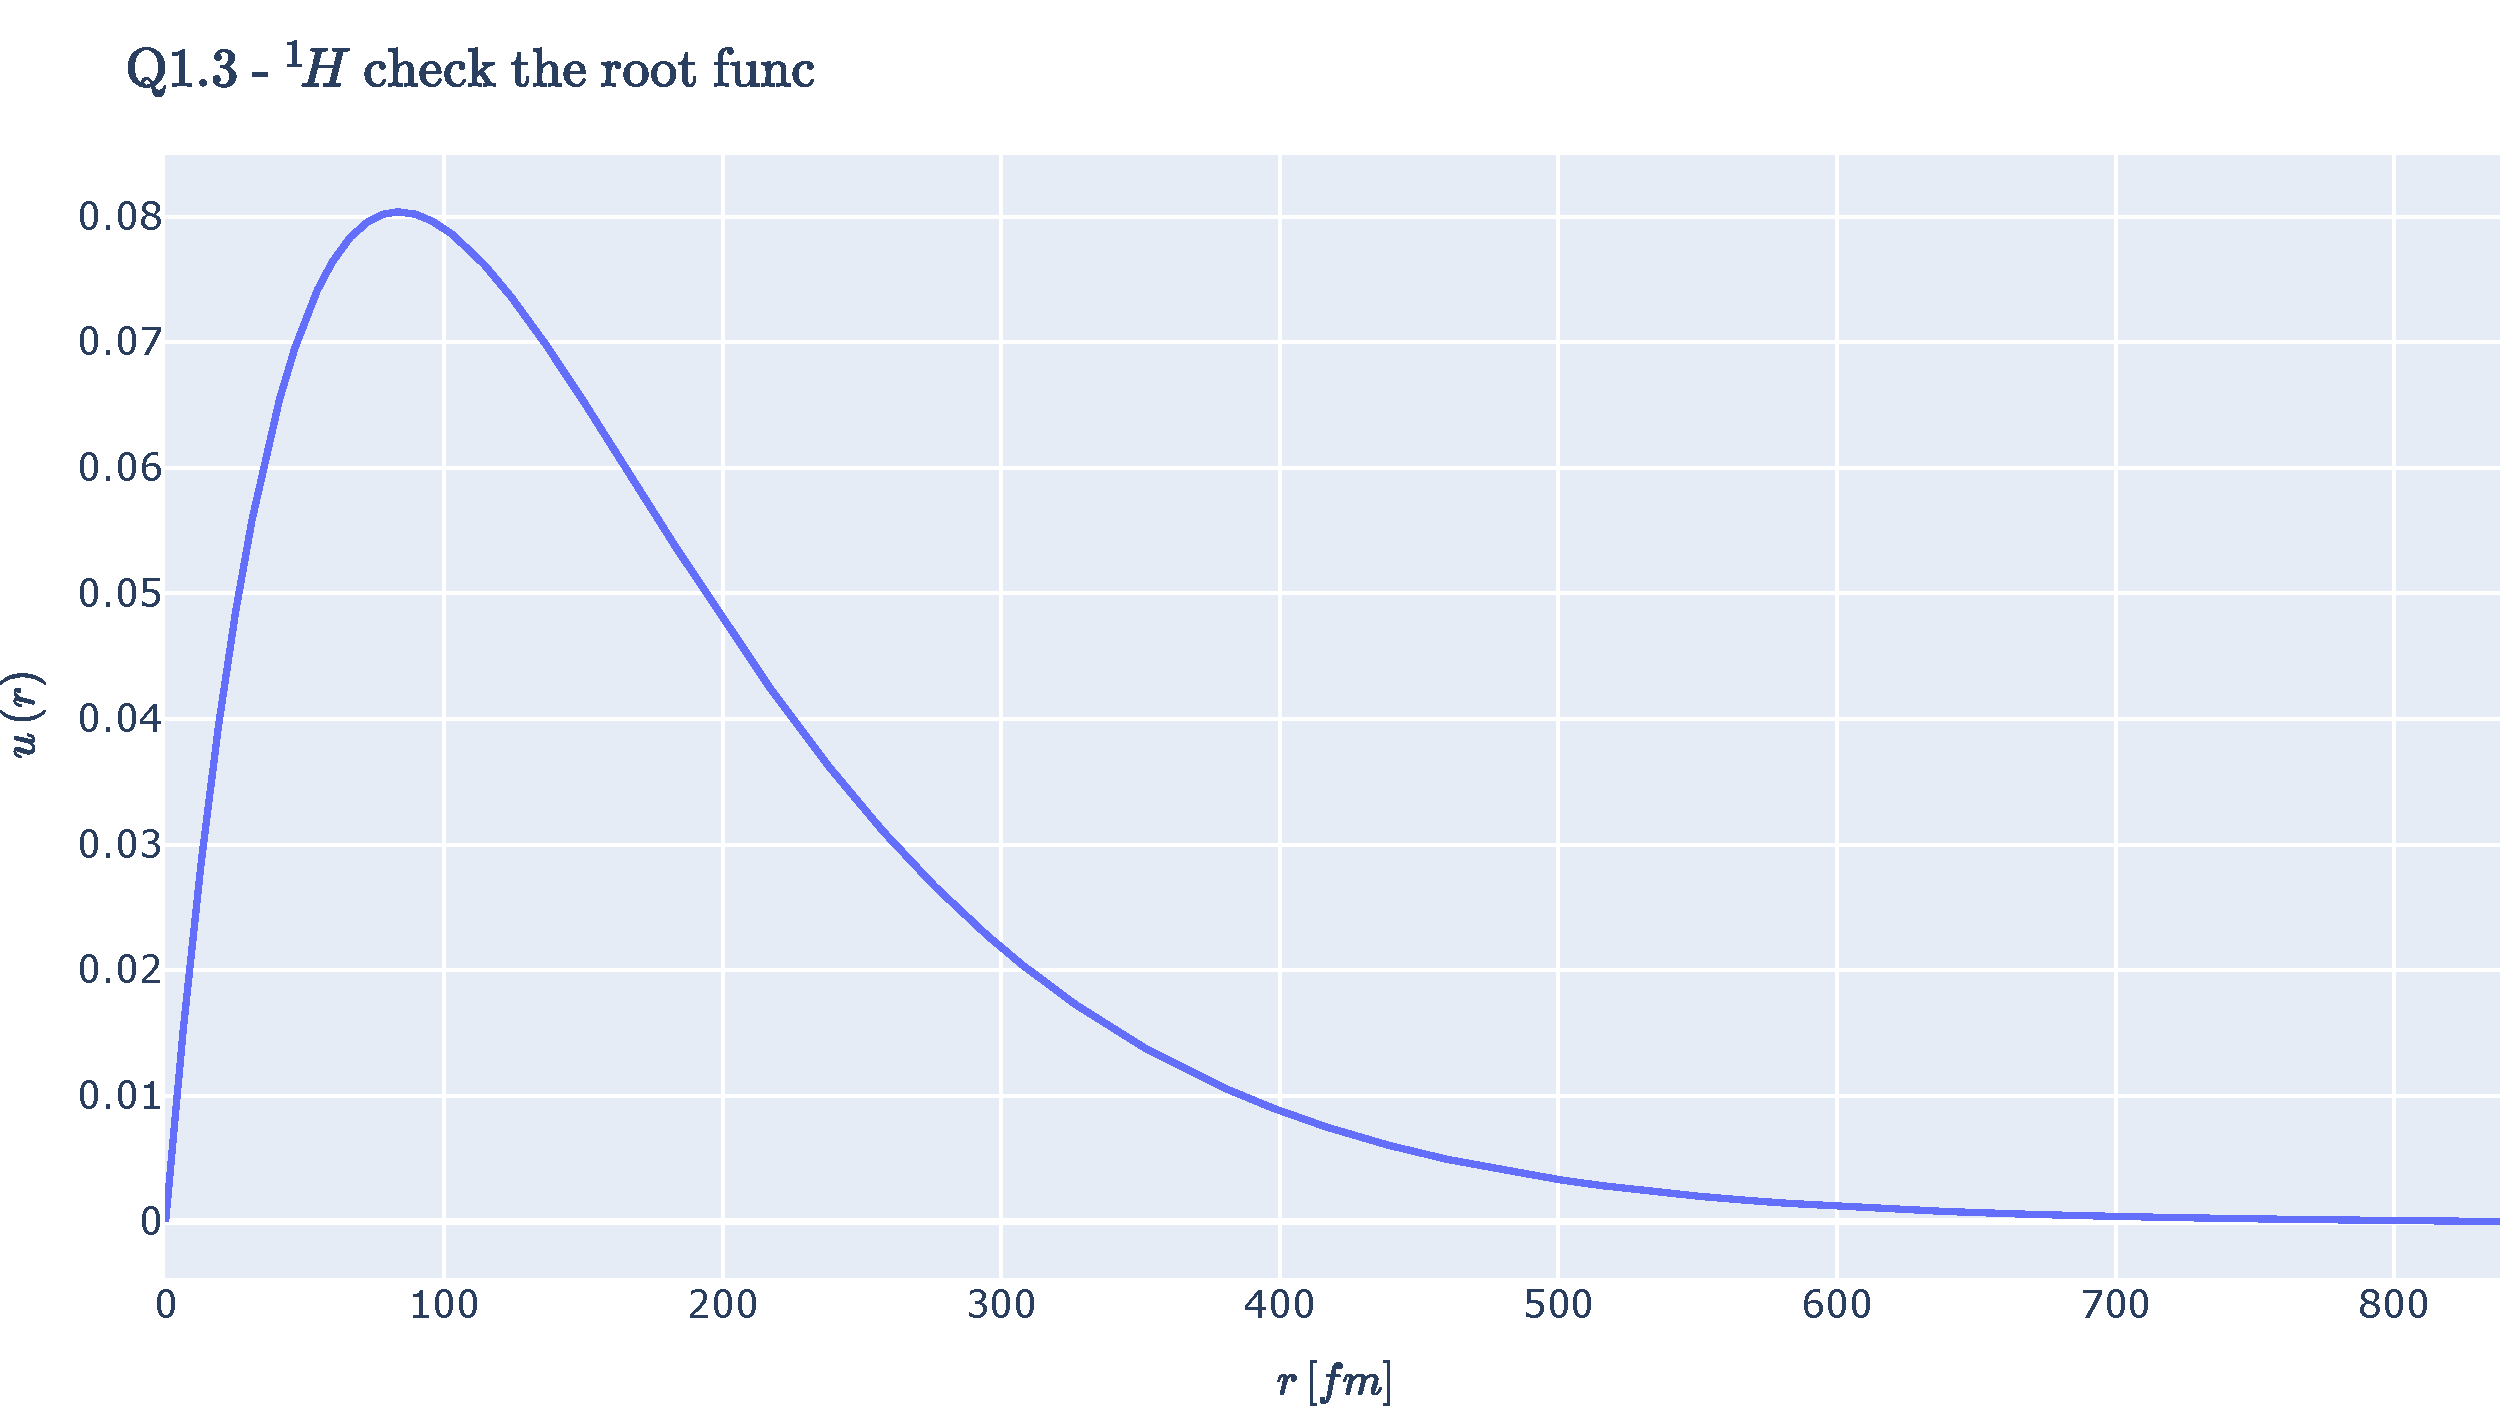
\includegraphics[width=\linewidth]{plots/1.3.pdf}
    \caption{פונקציית הגל עבור אנרגיה שנמצאה}
\end{figure}

\subsection{ההשפעה של מספר הנקודות N על הדיוק של הפתרון}
עבור הנתונים $R=20 a_B $ ועבור מספר משתנה של נקודות $N = 100, 1000, 10000, 100000$ ביצעתי את החישוב הנומרי לתחום האנרגיה של רמת היסוד (כמו ב\ref{subsec:1.2}). 
\begin{figure}[h]\label{fig:1.4}
    \centering
    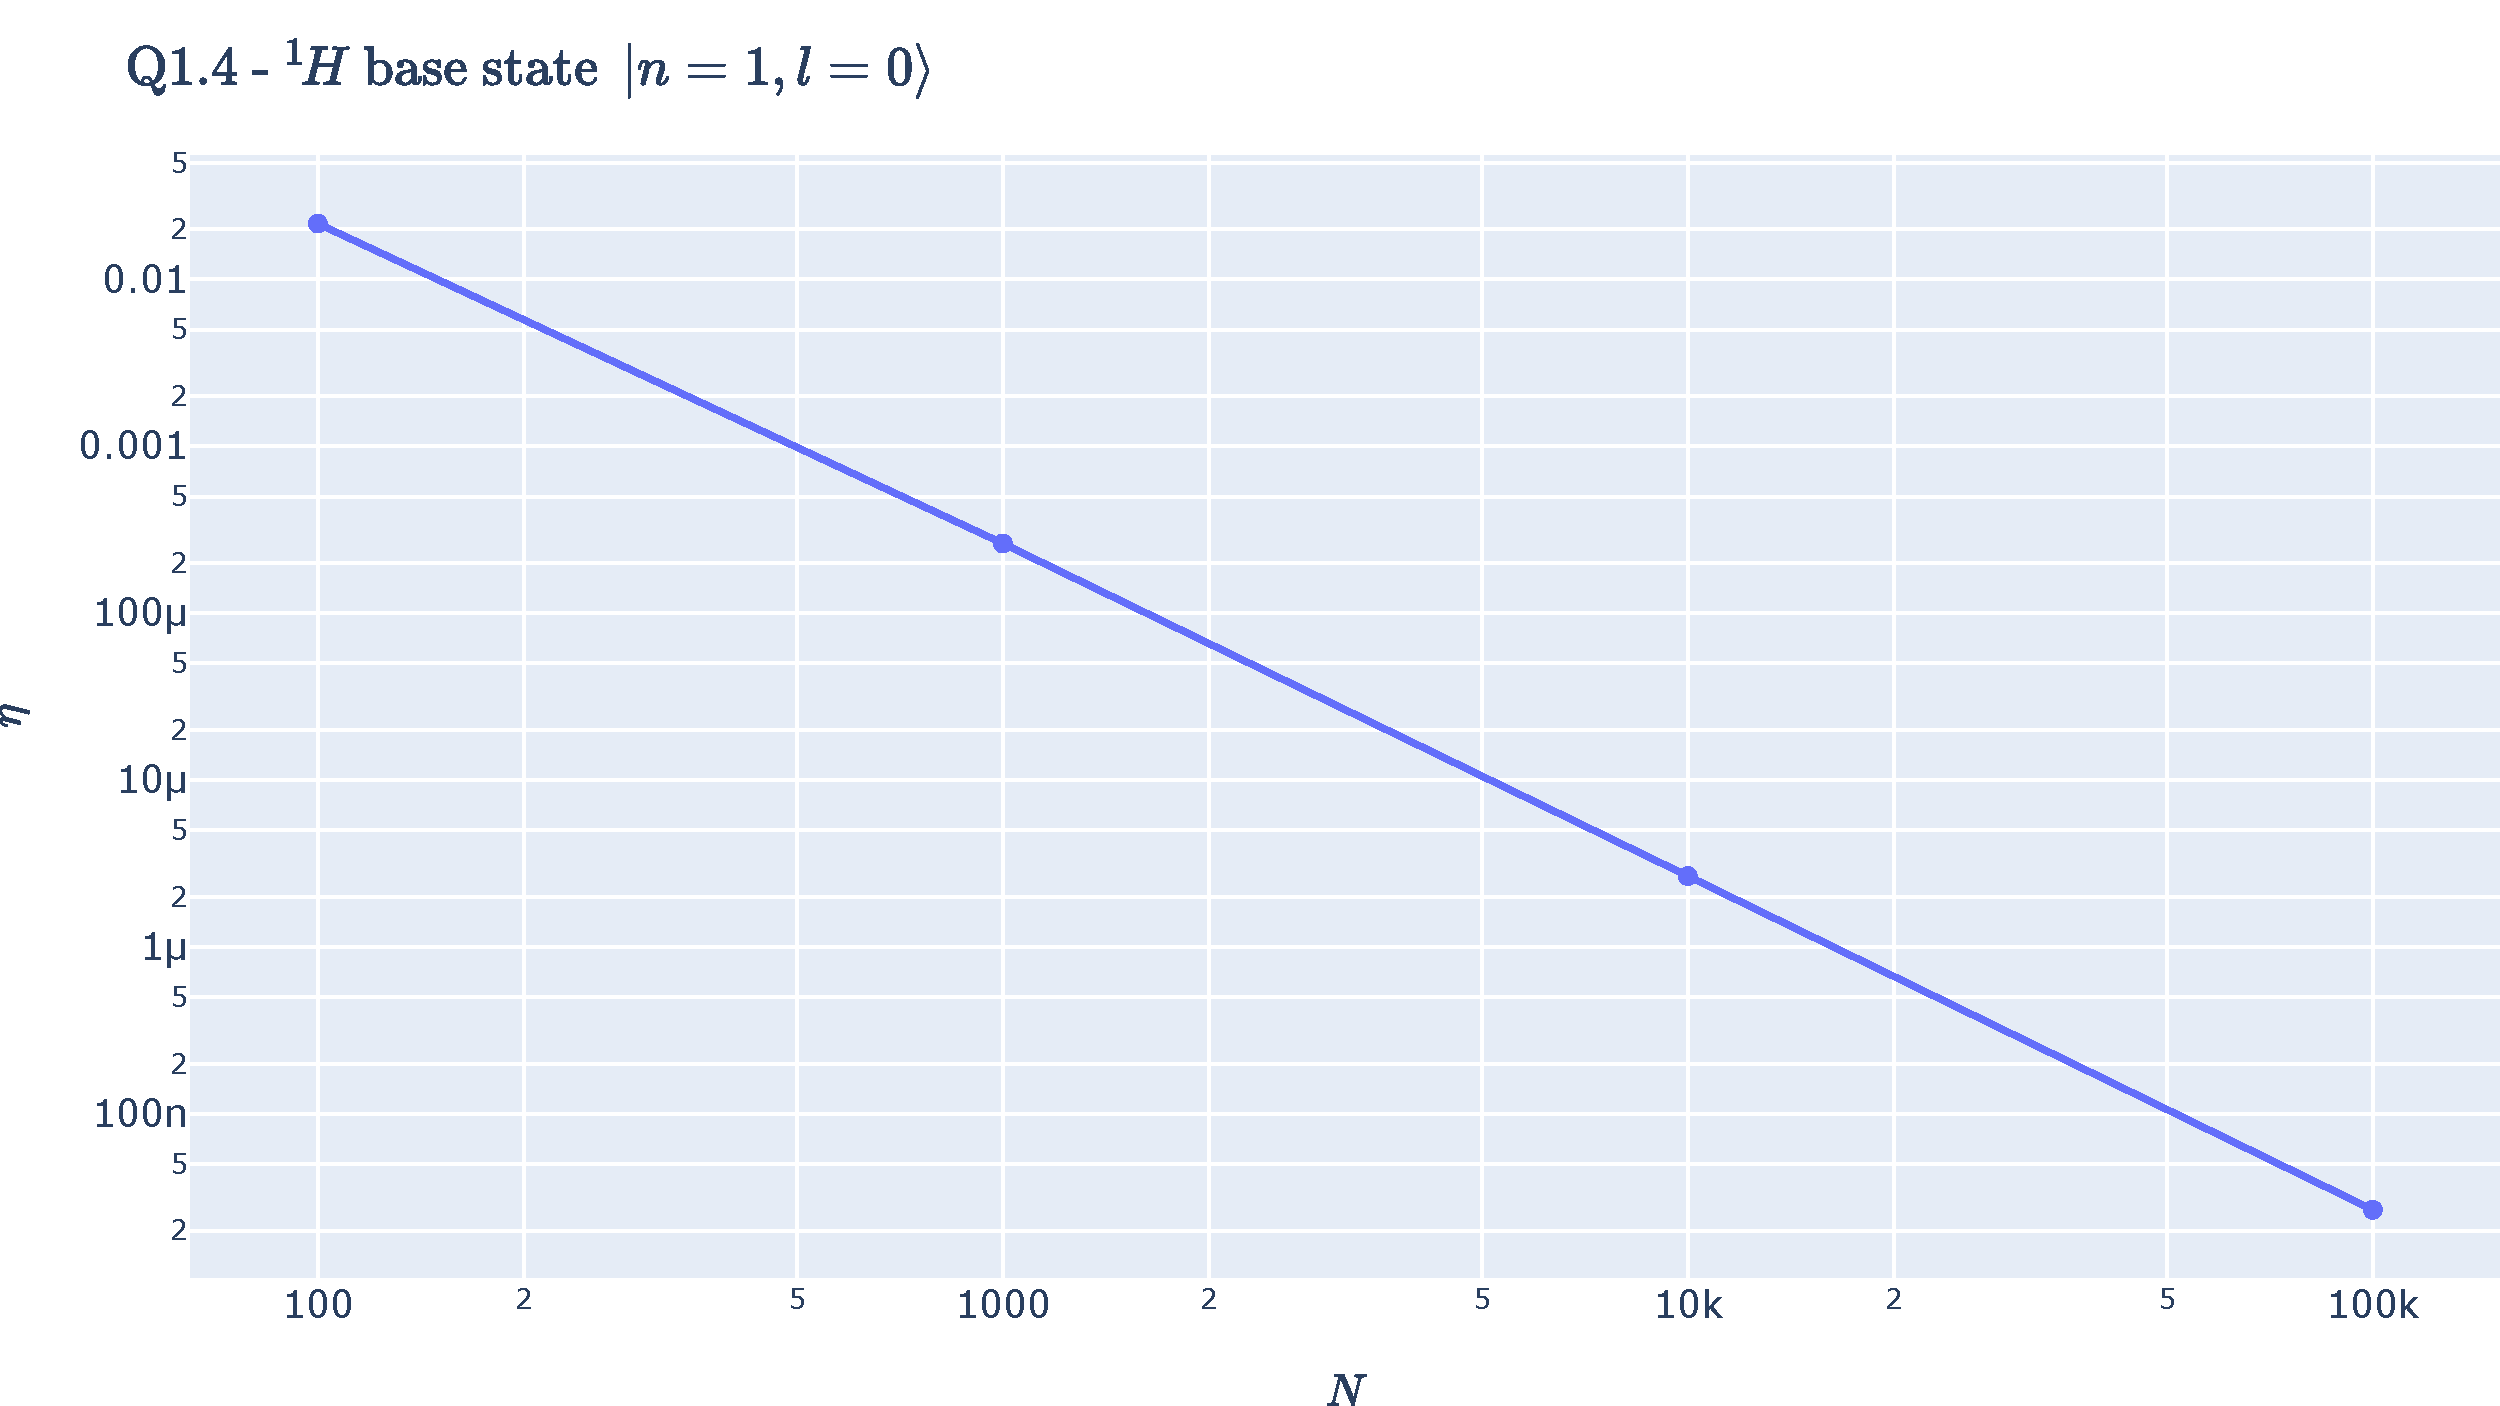
\includegraphics[width=\linewidth]{plots/1.4.pdf}
    \caption{השפעת מספר הנקודות על הדיוק של הפתרון}
\end{figure}


\end{document}
